\documentclass[12pt, twoside]{article}
\usepackage[letterpaper, margin=1in, headsep=0.5in]{geometry}
\usepackage[english]{babel}
\usepackage[utf8]{inputenc}
\usepackage{amsmath}
\usepackage{amsfonts}
\usepackage{amssymb}
\usepackage{tikz}
\usetikzlibrary{quotes, angles}
\usepackage{graphicx}
\usepackage{enumitem}
\usepackage{multicol}

\newif\ifmeta
\metatrue %print standards and topics tags

\title{Regents Geometry}
\author{Chris Huson}
\date{September 2020}

\usepackage{fancyhdr}
\pagestyle{fancy}
\fancyhf{}
\renewcommand{\headrulewidth}{0pt} % disable the underline of the header
\raggedbottom


\fancyhead[LE]{\thepage}
\fancyhead[RO]{\thepage \\ Name: \hspace{4cm} \,\\}
\fancyhead[LO]{BECA / Dr. Huson / Geometry \\* 1-9 Solving for angle measures}

\begin{document}

\subsubsection*{I can solve for angle measures}
\begin{enumerate}
\item Do Now: $m\angle ABD=30^\circ$, $m\angle DBC=45^\circ$. Find $m\angle ABC$.\vspace{0.5cm}
  \begin{flushright}
    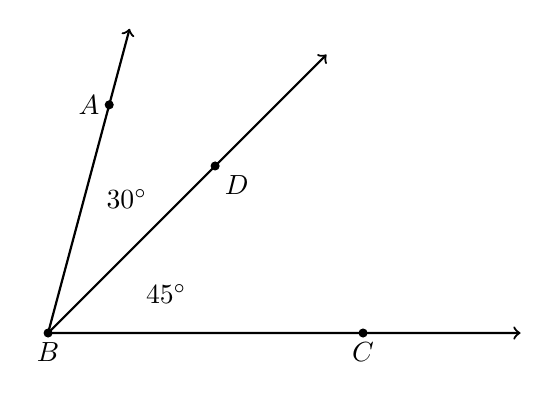
\begin{tikzpicture}
      \draw [<->, thick] (45:5)--(0,0)--(6,0);
      \draw [->, thick] (0,0)--(75:4);
      \draw [fill] (75:3) circle [radius=0.05] node[left]{$A$};
      \draw [fill] (45:3) circle [radius=0.05] node[below right]{$D$};
      \draw [fill] (0,0) circle [radius=0.05] node[below]{$B$};
      \draw [fill] (4,0) circle [radius=0.05] node[below]{$C$};
      \node at (1.5,0.5){$45^\circ$};
      \node at (1,1.7){$30^\circ$};
    \end{tikzpicture}
    \end{flushright}

\item Two lines intersect with $m\angle 1=80^\circ$. Find the measures of $\angle 2$, $\angle 3$, and $\angle 4$.
  \begin{flushleft}
  \begin{tikzpicture}[scale=0.8]
    \draw [<->, thick] (0,-1.5)--(10,1.5);
    \draw [<->, thick] (2,3.5)--(7,-3.5);
    \node at (2,.4){$m\angle 1=80^\circ$};
    \node at (6,-.6){3};
    \node at (5,1){2};
    \node at (4,-1){4};
    %\draw [fill] (0,0) circle [radius=0.05] node[below]{$P$};
    %\draw [fill] (6,0) circle [radius=0.05] node[below]{$R$};
    %\draw [fill] (3,0) circle [radius=0.05] node[below]{$Q$};
  \end{tikzpicture}
  \end{flushleft}

\item $\angle POQ$ and $\angle QOR$ are complementary angles. Given $m\angle POQ=51^\circ$, find $m\angle QOR$. \vspace{0.25cm}
  \begin{center}
  \begin{tikzpicture}[scale=1.2, rotate=0]
    \draw [->, thick] (0,0)--(129:4);
    \draw [<->, thick] (-5,0)--(5,0);
    \draw [->, thick] (0,0)--(0,4);
    \draw (0,0)++(0.3,0)--++(0,0.3)--+(-0.3,0);
    \draw [fill] (129:3) circle [radius=0.05] node[below left]{$Q$};
    \draw [fill] (-4,0) circle [radius=0.05] node[below]{$P$}; 
    \draw [fill] (0,0) circle [radius=0.05] node[below right]{$O$};
    \draw [fill] (0,3) circle [radius=0.05] node[right]{$R$};
    \node at (-1,0.4){$51^\circ$};
    \node at (-0.4,1.2){$x^\circ$};
  \end{tikzpicture}
  \end{center}

\newpage
\item Given $m\angle ADB=110^\circ$, $m\angle ADC = 75^\circ$, and $m\angle BDC = 3x+5$. Find $x$.
  \begin{enumerate}
    \begin{multicols}{2}
    \item Label the diagram.
    \item Write an equation.
    \item Solve for $x$. \vspace{3cm}

    \begin{flushright}
    \begin{tikzpicture}[scale=1.2]
      \draw [->, thick] (0,0)--(35:5);
      \draw [->, thick] (0,0)--(4,0);
      \draw [->, thick] (0,0)--(110:4);
      \draw [fill] (110:3) circle [radius=0.05] node[left ]{$A$};
      \draw [fill] (35:4) circle [radius=0.05] node[above left ]{$C$};
      \draw [fill] (0,0) circle [radius=0.05] node[left]{$D$};
      \draw [fill] (3,0) circle [radius=0.05] node[below]{$B$};
    \end{tikzpicture}
    \end{flushright}
  \end{multicols}
  \item Check your answer
  \end{enumerate} \vspace{2cm}
  

\item Points that are all located on the same line are $\rule{4cm}{0.15mm}$. \bigskip
\item Line segments that have the same length are $\rule{4cm}{0.15mm}$. \bigskip

\item Given $\overline{ABC}$, $AB=3.8$, and $BC=1.7$.
  \begin{enumerate}
    \item Find ${AC}$.\\[1.cm]
      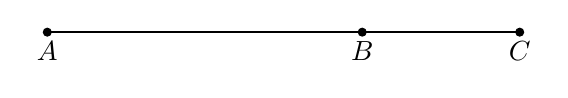
\begin{tikzpicture}
        \draw [-, thick] (1,0)--(7,0);
        \draw [fill] (1,0) circle [radius=0.05] node[below]{$A$};
        \draw [fill] (5,0) circle [radius=0.05] node[below]{$B$};
        \draw [fill] (7,0) circle [radius=0.05] node[below]{$C$};
      \end{tikzpicture} \vspace{1cm}
    \item The postulate used in this problem is the \rule{6cm}{0.15mm}.
  \end{enumerate}

\item Given $\overline{FG}$ as shown. What is the distance on the number line between the points?\\[20pt]
    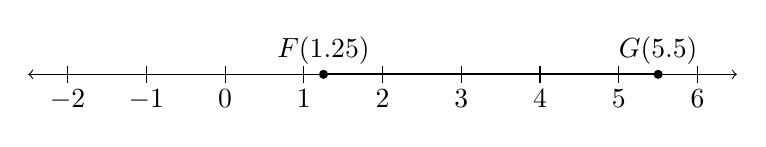
\begin{tikzpicture}
      \draw [<->] (-2.5,0)--(6.5,0);
      \foreach \x in {-2,...,6} %2 leading for diff!=1
        \draw[shift={(\x,0)},color=black] (0pt,-3pt) -- (0pt,3pt) node[below=5pt]  {$\x$};
        \draw [thick] (1.25,0)--(5.5,0);
        \draw [fill] (1.25,0) circle [radius=0.05] node[above] {$F(1.25)$};
        \draw [fill] (5.5,0) circle [radius=0.05] node[above] {$G(5.5)$};
    \end{tikzpicture}

\end{enumerate}
\end{document}